\chapter{Primal Formulation with Non-Linear Model}\label{chap: deep}

In Chapter~\ref{chap: framework} we introduced general framework for binary classification at the top samples, and showed multiple formulations that fall into it. All these formulations are summarized in Table~\ref{tab: summary formulations}. In Chapter~\ref{chap: linear}, we discussed theoretical properties of all formulations for special case of linear model. Since many real world problems are not lineary separable, in Chpater~\ref{chap: dual}, we derived dual forms of all formulations. Since these dual formulations are very similar to standard SVM, we incorporeted kernel trick to add non-linearity into our settings. Moreover, we derived efficient algorithm to solve these dual formulations. Even though we derived a way how to use non-linear model, the dual formulations are not suitable for large data. For this reason, in this chapter, we focus on the case, when the general model~$f$ is used, i.e. we have the following formulation
\begin{mini}{\bm{w}, \, t}{
  \frac{1}{2} \norm{\bm{w}}^2 + \lambda_1 \cdot \fps(\bm{s}, t) + \lambda_2 \cdot \fns(\bm{s}, t)
  }{\label{eq: aatp deep general}}{}
  \addConstraint{s_i}{= f(\bm{x}_i; \bm{w}), \quad i \in \I}
  \addConstraint{t}{= G\Brac{\bm{s}, \bm{y}},}
\end{mini}
where~$f$ is an arbitrary model. Since our goal is to derive method how to solve formulations from Table~\ref{tab: summary formulations} for large data, the model~$f$ can be for example some neural network. The standard way how to solve problems with neural networks is to use stochastic gradient descent. In such a case, the dataset is split into several small minibatches and at each iteration all operations are performed only on one small minibatch. For standard problems it can be performed seamlessly, since these problems are decomposable. However, the decision threshold~$s$ in our formulaion~\eqref{eq: aatp deep general} depends \emph{all} scores~$\bm{s}.$ Therefore, the objective is non-additive and non-decomposable. In the following text, we show how to modify stochastic gradient to prevent overcome this issue.

\section{Basic approach}

In this section we show a basic algorithm to solve any fromulation from Table~\ref{tab: summary formulations}. Since we want to use stochastic gradient descent, the whole section assumes that the classifier~$f$ is differentiable. The optimization problem~\eqref{eq: aatp deep general} depends on two decision variables~$\bm{w}$ and~$t.$ However, for all formulations from Table~\ref{tab: summary formulations} and for each~$\bm{w}$, the threshold~$t$ can be computed uniquely. We stress this dependence by writing~$t(\bm{w})$ instead of~$t$. By doing so, we effectively remove the threshold~$t$ from the decision variables and~$\bm{w}$ remains the only decision variable. Denoting the objective of~\eqref{eq: aatp deep general} by~$L(\bm{w})$
\begin{equation*}
  L(\bm{w})
    = \frac{1}{2}\norm{\bm{w}}^2 + \frac{1}{\npos} \sum_{i \in \Ipos} l \Brac{t(\bm{w}) - f(\bm{x}_i; \bm{w})},
\end{equation*}
the chain rule implies that the gradient is equal to
\begin{equation}\label{eq:grad1}
  \nabla L(\bm{w})
    = \bm{w} + \frac{1}{\npos} \sum_{i \in \Ipos} l'\Brac{t(\bm{w}) - f(\bm{x}_i; \bm{w})}\Brac{\nabla t(\bm{w}) - \nabla f(\bm{x}_i; \bm{w})}.
\end{equation}
The only remaining part is the computation of~$\nabla t(\bm{w})$. It is simple for most of the formulations from Table~\ref{tab: summary formulations}. Moreover, Theorem~\ref{thm: differentiability} shows the computation for \PatMat. The stochastic gradient descent replaces the sum over all positive samples~$\Ipos$ with a sum over all positive samples in a minibatch~$\Imbpos$. However, since the threshold~$t$ depends on all scores~$\bm{s}$, it needs to be approximated on the minibatch as well. The most straightforward way is to use the same rule as for the whole dataset and compute the samplesd threshold~$\hat{t}$ only on data from the minibatch. Denoting the number of positive samples in the minibatch by~$\nmbpos$, we replace the true gradient with
\begin{equation}\label{eq:grad2}
  \nabla \hat{L}(\bm{w})
    = \bm{w} + \frac{1}{\nmbpos} \sum_{i \in \Imbpos} l'\Brac{\hat{t}(\bm{w}) - f(\bm{x}_i; \bm{w})}\Brac{\nabla \hat{t}(\bm{w}) - \nabla f(\bm{x}_i; \bm{w})}.
\end{equation}
However, when the threshold is computed on a minibatch, it provides a lower estimate of the true threshold. Therefore, the sampled threshold is a biased estimate of the true threshold. Figure~\ref{fig:thresholds1} illustrates this phenomenon. The bias between the true and sampled thresholds is large even for medium-sized minibatches. Backpropagation then propagates this sampling error through the whole gradient, and consequently, the minibatch gradient is a biased estimate of the true gradient. This brings numerical issues~\cite{bottou2018optimization}. Nveretheles, we summarize the procedure described above in Algorithm~\ref{alg: deep basic}.

\begin{figure}
  \centering
  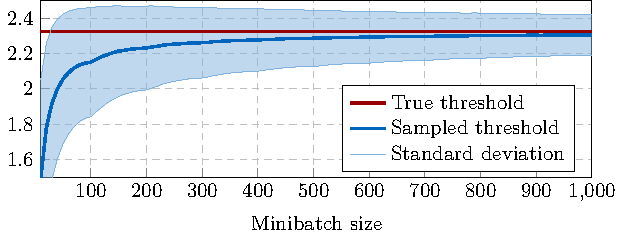
\includegraphics[width = \linewidth]{images/deep_threshold_bias.pdf}
  \caption{The bias between the sampled and true thresholds computed from scores following the standard normal distribution. The threshold separates the top~$1\%$ of samples with the highest scores.}
  \label{fig:thresholds1}
\end{figure}

\begin{algorithm}
  \centering
  \begin{algorithmic}[1]
    \State Initialize weights~$\bm{w},$ stepsiz~$\alpha$
    \Repeat
    \State Select minibatch~$\Imb$
    \State Compute~$s_i \gets f(\bm{w};\bm{x}_i)$ for all~$i \in \Imb$
    \State Set~$\hat{t} \gets G(\bm{s}_{\text{mb}}, \bm{y}_{\text{mb}})$
    \State Compute~$\nabla \hat{L}$ based on~$\Imb$
    \State Make a gradient~$\bm{w} \gets \bm{w} - \alpha \cdot \nabla \hat{L}$
    \Until{stopping criterion is satisfied}
  \end{algorithmic}
  \caption{Basic algorithm for solving~\eqref{eq: aatp deep general}}
  \label{alg: deep basic}
\end{algorithm}

\subsection{Bias of Sampled Gradient}

Convergence proofs of the stochastic gradient descent require that the sampled gradient is an unbiased estimate of the true gradient~\cite{bottou2018optimization}. This means that
\begin{equation}\label{eq:defin_bias}
  \bias(\bm{w}) := \nabla L(\bm{w}) - \EE \nabla \hat{L}(\bm{w})
\end{equation}
equals to~$0$ for all~$\bm{w}$. A comparison of \eqref{eq:grad1} and \eqref{eq:grad2} shows that a necessary condition is that the sampled threshold~$\hat{t}$ is an unbiased estimate of the true threshold~$t$. However, the sampled version underestimates the true value, which is evident for \TopPush where the sampled maximum is always smaller or equal to the true maximum. The next result quantifies the difference between the sampled and true thresholds.

\begin{proposition}[\cite{glynn1996importance}]\label{proposition:bound}
  Consider an absolutely continuous random variable~$X$ with distribution function~$F.$ Let $X_1,\, X_2, \ldots, \, X_n$ be iid samples from~$X$ and let~$\tau \in (0,1).$ Denote the true threshold
  \begin{equation*}
    t = F^{-1}(1 - \tau),
  \end{equation*}
  and the sampled threshold~$\hat{t} = X_{[\lceil n\tau\rceil]}$. If~$F$ is differentiable with a positive gradient at~$t$, then
  \begin{equation*}
    \sqrt{n}\Brac{t - \hat{t}} \rightarrow \mathcal{N} \Brac{0, \; \frac{\tau(1-\tau)}{F'(t)^2}},
  \end{equation*}
  where the convergence is in distribution and~$\mathcal{N}$ denotes the normal distribution.
\end{proposition}

This proposition states that when the minibatch size increases to infinity, the variance of the sampled threshold is approximately
\begin{equation*}
  \frac{\tau(1-\tau)}{nF'(t)^2}.
\end{equation*}
Figure~\ref{fig:thresholds1} shows this empirically for the case where the scores follow the standard normal distribution and~$\tau=0.01$ is the desired top fraction of all samples. The approximation is poor with both large bias and standard deviation. The natural choice to mitigate the bias is to work with large minibatches. Even though this is not a standard way, some works suggest this route~\cite{you2019large}. When the minibatch is large, it contains more samples and the sampled threshold is more precise. This approach is applicable to any method from Table~\ref{tab: summary formulations}.

\section{DeepTopPush and DeepTopPushK}

In the rpevious chapter we presented a basic way how to modify stochastic gradient descent to work for formulations from Table~\ref{tab: summary formulations}. However, this approach provides biased gradient and the only way how to reduce the biass is to use large minibatches. But various reasons may enforce the use of small minibatches. In this section we derive a new method called \DeepTopPush, that mitigates this bias in different way.

Our new method is based on method presented in~\cite{li2014top} that is called \TopPush. Since we use the same formulation as \TopPush but assume an arbitrary model~$f$, we name it \DeepTopPush. Authors of~\cite{li2014top} proposed the \TopPush formulation with linear model and solved it in its dual form. In Section~\ref{sec: ranking} we generalized this formulation for general model~$f,$ and in Chapter~\ref{chap: linear} we solved the formulation directly in its primal form for linear classifiers. For general model~$f,$ we stay in the primal form to be able to employ stochastic gradient descent. It means that we have the following optimization problem
\begin{mini}{\bm{w}, \, t}{
  \frac{1}{\npos} \fn(\bm{s}, t)
  }{\label{eq: toppush deep}}{}
  \addConstraint{s_i}{= f(\bm{x}_i; \bm{w}), \quad i \in \I}
  \addConstraint{t}{= s_{[1]}^-.}
\end{mini}
Due to non-decomposability, we need to propose a way of computing the gradient and reduce the bias mentioned above. Since the threshold always equals to one of the scores~\cite{boyd2012accuracy}, its computation has a simple local formula. In other words, if the highest negative score~$s_{[1]}^-$ corresponds to sample~$\bm{x}_{j^{\star}}$ with index~$j^{\star},$ then the gradient equals
\begin{equation*}
  \nabla t = f(\bm{x}_{j^{\star}}; \bm{w})
\end{equation*}
The core idea of \DeepTopPush is a modification of the idea presented in~\cite{adam2019machine}. When the weights~$\bm{w}$ of model~$f$ are updated using stochastic gradient descent, the scores~$\bm{s}$ usually do not change much. It is true especially for a small learning rates. This means that if a sample has the highest score, it will likely have the highest score even after the gradient step. Since the threshold~$t$ for \TopPush equals the highest score corresponding to negative samples, we can easily track to which sample this score corresponds. Therefore, we can enhance the current minibatch by the sample that represents the treshold in the previous minibatch. This significantly increases the chance that the sampled threshold is the true threshold. The whole procedure is summarized in Algorithm~\ref{alg2}. In every iteration, it stores the index~$j^{\star}$ of the sample, which equals the threshold (step~7). We add it to the enhanced minibatch (step 4). Since we can track only the maximum, we set the threshold as the maximum of scores from negative samples (step~6) and minimize false-positives.

\begin{algorithm}[H]
  \centering
  \begin{algorithmic}[1]
    \State Initialize weights~$\bm{w}$, random index~$j^{\star}$
    \Repeat
    \State Select minibatch~$\Imb$
    \State Enhance minibatch~$\Imbenh = \Imb \cup \{j^{\star}\}$
    \State Compute~$s_i \gets f(\bm{w};\bm{x}_i)$ for~$i\in\Imbenh$
    \State Set~$\hat{t} \gets \{\max s_i \mid i \in \Imbenh \cap I^-\}$
    \State Find index~$j^{\star}$ such that~$t = s_{j^{\star}}$
    \State Compute~$\nabla \hat{L}$ based on~$\Imbenh \cap I^+$
    \State Make a gradient step
    \Until{stopping criterion is satisfied}
  \end{algorithmic}
  \caption{DeepTopPush as an efficient method for maximizing accuracy at the top.}
  \label{alg2}
\end{algorithm}

\subsection{Bias of Sampled Gradient}

Even though this result gives us insight into the bias of the sampled threshold, we are ultimately interested in the bias of the sampled gradient~$\nabla \hat{L}(\bm{w})$. To do so, recall that~$j^{\star}$ is the threshold index on the whole dataset ($t=z_{j^{\star}}$) while~$\hat j$ is the threshold index on the minibatch ($\hat{t}=z_{\hat j}$). We split the computation based on whether these two indices are identical.

\begin{restatable}{lemma}{lemmacovergencedeep}\label{lemma:convergence}
  Let~$j^{\star}$ be unique. Assume that the selection of positive and negative samples into the minibatch is independent and that the threshold is computed from negative samples while the objective is computed from positive samples. Then the conditional expectation of the sampled gradient satisfies
  \begin{equation*}
    \EE\Brac{\nabla \hat{L}(\bm{w}) \mid \hat j=j^{\star}} =  \nabla L(\bm{w}).
  \end{equation*}
\end{restatable}

Now we present the main result about the bias.

\begin{restatable}{theorem}{thmcovergencedeep}\label{theorem:convergence}
  Under the assumptions of Lemma~\ref{lemma:convergence}, the bias of the sampled gradient from \eqref{eq:defin_bias} satisfies
  \begin{equation}\label{eq:comp_bias}
    \bias(\bm{w}) = \PP(\hat j\neq j^{\star}) \Brac{\nabla L(\bm{w}) - \EE\Brac{\nabla \hat{L}(\bm{w}) \mid \hat j\neq j^{\star}}}.
  \end{equation}
\end{restatable}

The assumptions of Theorem~\ref{theorem:convergence} holds for all methods from Table~\ref{table:summary} with the exception of Rec@K. For this method, the bias contains an additional term, as we show in the appendix.

The bias \eqref{eq:comp_bias} consists of a multiplication of two terms. We propose two strategies for reducing the bias. The first strategy reduces both terms, while the second strategy reduces only the first term.

\subsection{Bias reduction}\label{sec:bias2}

The natural choice to mitigate the bias is to work with large minibatches. Even though this is not a standard way, some works suggest this route~\cite{you2019large}. When the minibatch is large, it contains more samples and the chance that~$\hat j$ differs from~$j^{\star}$ decreases. This reduces the first term in~\eqref{eq:comp_bias}. Moreover, Proposition~\ref{proposition:bound} ensures that the difference between the sampled threshold~$\hat{t}$ and the true threshold~$t$ is small. Then the difference between the true gradient \eqref{eq:grad1} and the sampled gradient \eqref{eq:grad2} decreases as well. This reduces the second term in \eqref{eq:comp_bias}. This approach is applicable to any method from Table~\ref{table:summary}.
